%% LaTeX template for BSc Computing for Games final year project dissertations
%% by Edward Powley
%% Games Academy, Falmouth University, UK

%% Based on:
%% bare_jrnl.tex
%% V1.4b
%% 2015/08/26
%% by Michael Shell
%% see http://www.michaelshell.org/
%% for current contact information.
%%
%% This is a skeleton file demonstrating the use of IEEEtran.cls
%% (requires IEEEtran.cls version 1.8b or later) with an IEEE
%% journal paper.
%%
%% Support sites:
%% http://www.michaelshell.org/tex/ieeetran/
%% http://www.ctan.org/pkg/ieeetran
%% and
%% http://www.ieee.org/

%%*************************************************************************
%% Legal Notice:
%% This code is offered as-is without any warranty either expressed or
%% implied; without even the implied warranty of MERCHANTABILITY or
%% FITNESS FOR A PARTICULAR PURPOSE! 
%% User assumes all risk.
%% In no event shall the IEEE or any contributor to this code be liable for
%% any damages or losses, including, but not limited to, incidental,
%% consequential, or any other damages, resulting from the use or misuse
%% of any information contained here.
%%
%% All comments are the opinions of their respective authors and are not
%% necessarily endorsed by the IEEE.
%%
%% This work is distributed under the LaTeX Project Public License (LPPL)
%% ( http://www.latex-project.org/ ) version 1.3, and may be freely used,
%% distributed and modified. A copy of the LPPL, version 1.3, is included
%% in the base LaTeX documentation of all distributions of LaTeX released
%% 2003/12/01 or later.
%% Retain all contribution notices and credits.
%% ** Modified files should be clearly indicated as such, including  **
%% ** renaming them and changing author support contact information. **
%%*************************************************************************


\documentclass[journal]{IEEEtran}

\usepackage{listings}
\usepackage{graphicx}
% Insert additional usepackage commands here
\graphicspath{ {Figures/} }
\usepackage{float}
%\usepackage{wrapfig}
\usepackage{amsmath}
%\usepackage[linesnumbered,ruled]{algorithm2e}
\usepackage{xargs}                      % Use more than one optional parameter in a new commands
\usepackage[pdftex,dvipsnames]{xcolor}  % Coloured text etc.
\usepackage{todonotes}
\usepackage{algpseudocode}
%\usepackage{algorithm}% http://ctan.org/pkg/algorithms

\begin{document}
%
% paper title
% Titles are generally capitalized except for words such as a, an, and, as,
% at, but, by, for, in, nor, of, on, or, the, to and up, which are usually
% not capitalized unless they are the first or last word of the title.
% Linebreaks \\ can be used within to get better formatting as desired.
% Do not put math or special symbols in the title.
\title{ How Does Visualising Path-finding in a NPC Affect How Players Explore a Game Level?}
%
%
% author name
\author{Madeleine Kay}

% The paper headers -- please do not change these, but uncomment one of them as appropriate
% Uncomment this one for COMP320
%\markboth{COMP320: Research Review and Proposal}{COMP320: Research Review and Proposal}
% Uncomment this one for COMP360
 \markboth{COMP360: Dissertation}{COMP360: Dissertation}

% make the title area
\maketitle

% As a general rule, do not put math, special symbols or citations
% in the abstract or keywords.
\begin{abstract}
% Opening: 
	This paper will look at the use of path-finding and \textit{Artificial Intelligence} (AI) visualisation in digital games.   Specifically at the use of foregrounding AI and the visualisation of path-finding. 
%	Challenge: 
While previous papers have researched AI visualisation and how to achieve it there did not appear to be many papers on the field of visualising AI in video games. There has been research into the visualisation of path-finding. However, the focus was most commonly on the use of visualisation in game design. 
% Action: 
	This paper looks at visualising various methods of path-finding on enemy NPCs in a 3D metroidvania game developed in Unity.\\
%Resolution:
 \todo[inline]{Analysis of the results showed that...}

\end{abstract}

\section{Introduction} \label{introduction}
\IEEEPARstart{T}{his} project will look at visualising the path-finding of an enemy \textit{Non Player Character} (NPC) using \textit{Rapidly-exploring Random Tree} (RRT) path-finding.  Figure~\ref{KuffnerRRT} shows an example of RRT path-finding. Here the RRT explores the area and then draws a path along the tree between the start and the goal nodes~\cite{Kuffner2000}. 

This paper will look at visualising the tree produced by RRT and the process taken to produce it. The visualisation will be around an enemy NPC. This will allow the players to see where the enemy NPC is going and what their line of sight is. 

Implementation of the visualisation will be in a level of a 3D game made in Unity 5.6\footnote[1]{Unity 5.6 Available: https://unity3d.com/get-unity/download/archive}. Logging tools in the play testing software will  the amount of time the players spends in a level and what percent of the level they explore. Analysis of this data will then determine whether the visualisation has had any affect on how participants explore.

Previous papers have researched visualising~\textit{Artifical Intelligence} (AI) and foregrounding AI. However, there is little on what effect this has on how the players explore the game.
The research question proposed in this project is: how does visualising RRT path finding in a NPC affect how a player explores a game level?

\section{Related Work} \label{RelatedWork}
As the focus of this paper is on path-finding that was the first area researched. The methods looked at were A* path-finding in section \ref{A*PF} and RRT path-finding in section \ref{RRTadnPathfinding}.  After that Foregrounding and Visualising AI was researched in section \ref{VisualisingAI}. While there is research on AI visualisation there was a lack of it for digital games and what research was on games often focused on game development and level design as can be seen in section \ref{VisualisingAI}. 

The literature review .... not many papers on the field of AI visualisation in digital games. 
\todo[inline]{EXPLAIN NOT MUCH IN FIELD ON GAMES MAKING THIS 'NEEDED'}



\subsection{A* Path-finding} \label{A*PF}
A* path-finding is widely used in both robotics and digital games~\cite{Algfoor2015}. In games A* appears to be the most commonly used path-finding algorithm~\cite{Algfoor2015}.

Hart~\textit{et al}~\cite{Hart1968} first proposed A* path-finding in 1968 as an improvement on Dijkstra's algorithm. A* aims to expand the fewest nodes possible to minimise the cost of the path where the cost is the distance between the start and  goal nodes. Figure \ref{A*Pseudo} shows pseudo-code for implementing A*. 

\begin{figure}[H]
	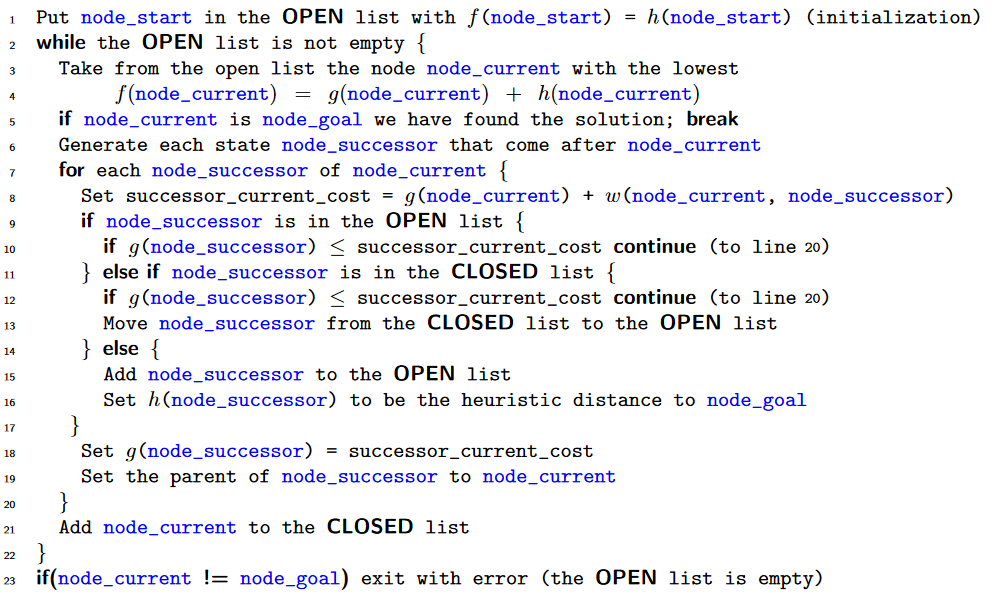
\includegraphics[width=1.0\linewidth]{APseudocode.png}
	\caption{Pseudo-code for A* path-finding~\cite{Hart1968}~\cite{pseudocode:A*}.}
	\label{A*Pseudo}
\end{figure} 

Algfoor~\textit{et al}~\cite{Algfoor2015} surveyed numerous papers on path finding. Their focus was on the use of different grid shapes in path-finding and the numerous algorithms available~\cite{Algfoor2015}. The most popular being the A* algorithm for use in both digital games and robotics. They surveyed many grid types and gave the advantages of each. 

Nash \textit{et al}~\cite{Nash2007} say that A* can not always find the true shortest path as it is limited to the grid. The shortest path can be found A* with post-smoothing paths or by using A* variants such as Theta*~\cite{Nash2007,Firmansyah2016}. Theta* expands on A* as it allows for all edges and angles in the grid to be used. Therefore, a path with a more optimal distance can be found.

While their focus is on Android games Firmansyah~\textit{et al}~\cite{Firmansyah2016} compared A* with Theta*. They found that performed similarly time wise. However, A* produced a path with less nodes expanded and Theta* produced a shorter path. 

Hu~\textit{et al}~\cite{Hu2012} propose an implementation of A* path-finding in the Unity engine, the engine used in this project.  While their implementation is in an older version Unity the implementation in Unity 5.6 should still be similar. A further paper on path-finding is Wang and Lu's~\cite{wang2012} paper which looks at path-finding in a 3-Dimensional environment. While again they were using A* they look at using A* in 3D and suggest using nodes instead of a grid.

Tremblay~\textit{et al}~\cite{Tremblay2014} look at the use of path-finding algorithms in level design. They compared 2-Dimensional A*, 3-Dimensional A*, RRT using A* for motion planning, RRT using \textit{Monte Carlo Tree Search} (MCTS) and MCTS alone. 2-Dimensional A* consistently gave the fastest result with the highest success rate. As this was for game level design instead of game play they ran the algorithms 1000 times on high specification computers. When used in this project the algorithms will only be run once however as A* in 2 dimensions had a 100 percent success rate this should not be an issue. 

\subsection{RRT and Pathfinding} \label{RRTadnPathfinding}
RRTs are a search method used more in robotics than in digital games~\cite{LaValle1998,Kuffner2000}. Kuffner and LaValle~\cite{Kuffner2000} first proposed RRT in 2000. They intended to produce a random algorithm more efficient than the other search algorithms available at the time.  Figure~\ref{KuffnerRRT} shows Kuffner and LaValle's~\cite{Kuffner2000} RRT Path Planner. Path Planner is a variant of RRT which has the intended use of finding paths from the generated tree.

\begin{figure}[h]
	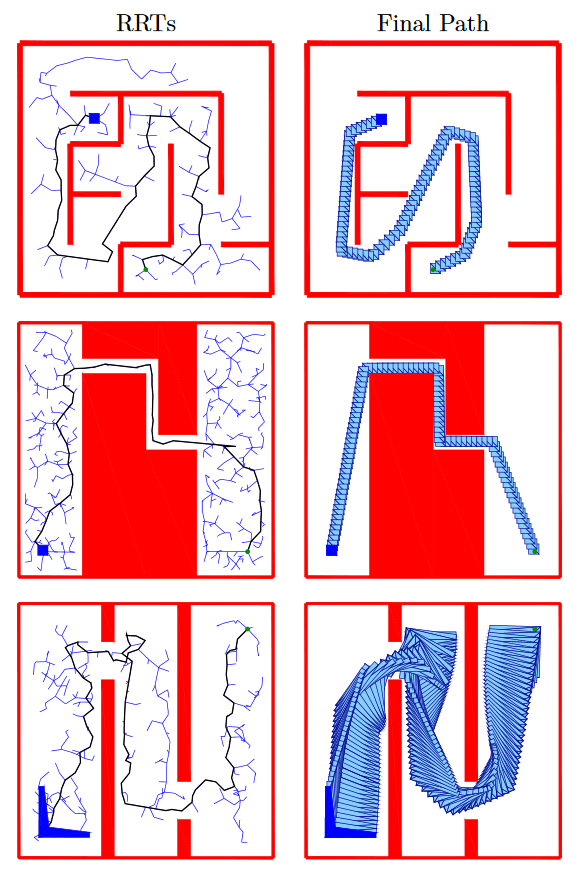
\includegraphics[width=1.0\linewidth]{KuffnerRRT.png}
	\caption{ Kuffner and LaValle's RRT path planner building a tree and plotting a path through it~\cite{Kuffner2000}.}
	\label{KuffnerRRT}
\end{figure} 

\todo[inline]{PSEUDOCODE FOR RRT}

%\begin{algorithmic}
%	\For{$k$ \gets $1$ to $K$} 
	
%	\EndFor
%\end{algorithmic}


The process for RRT involves the random placement of nodes. A parent is then selected by finding the closest pre-existing node~\cite{Kuffner2000}. Figure~\ref{RRTPseudocode} shows the pseudo-code for the RRT algorithm. 

\begin{figure}[h]
	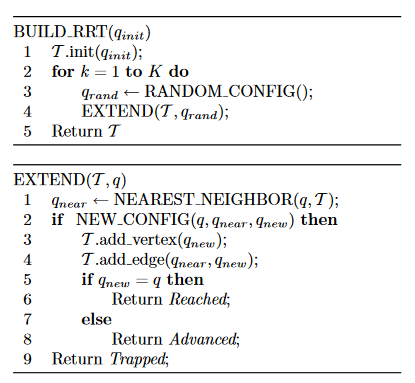
\includegraphics[width=1.0\linewidth]{RRTPseudocode.png}
	\caption{ Kuffner and LaValle's RRT algorithm pseudo-code for RRT construction~\cite{Kuffner2000}.}
	\label{RRTPseudocode}
\end{figure} 

RRTs goal is to find a path between two points with no collisions. The path found may not be the optimal path though~\cite{Kuffner2000,Karaman2011}. Karaman and Sertac~\cite{karaman2010} say that the chance of RRT finding an optimal path is very unlikely~\cite{karaman2010,Tremblay2014}.  Karaman \textit{et al} propose a variant of RRT called RRT*. RRT* starts the same as RRT, however, when a new node has to choose a parent node instead of selecting the nearest node it evaluates the cost of the nodes in regards to reaching its goal. Each iteration re-evaluates the parent nodes to reduce the cost. Rewiring of the tree happens when a lower cost path is found.

\subsection{Path-finding} \label{Pathfinding}
Bauer and Popovic~\cite{bauer2012} use RRT for level design in digital games. Like other papers mentioned in section \ref{VisualisingAI} they visualise the data to aid users~\cite{bauer2012,Haworth2010}. This data visualisation is for use in game development to aid game developers or to analyse procedurally generated levels. 

\begin{figure}[h]
	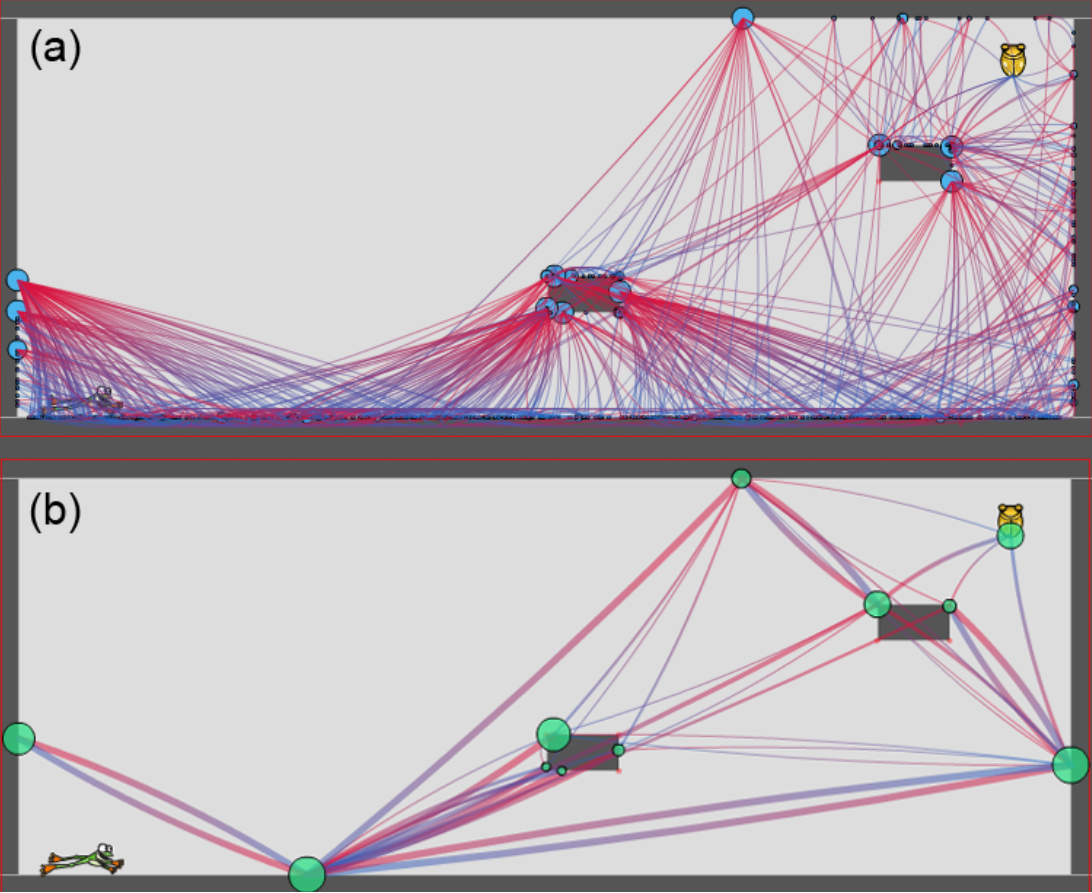
\includegraphics[width=1.0\linewidth]{BauerRRT.png}
	\caption{ Bauer \textit{et al}'s\cite{bauer2012} graph-based representation of RRT with and without clustering.}
	\label{BauerRRT}
\end{figure} 

Their focus is on level design not game-play. They propose a tool that analyses a level generated by PCG or a level designer. They then use RRT to calculate possible routes the player could take when playing.  Figure~\ref{BauerRRT} shows the output of the tool once it has been run on a basic level design.  The first image, image a, may be difficult to read. So, they make use of Dongen's method for graph clustering to make the output more legible as shown in the second image, image b~\cite{bauer2012,Dongen2001}.  

The focus of this project is on a similar type of visualisation but running in the game instead of during the game development. Therefore, there is a need for a similar technique to cluster the output of RRT. This should make the visualisation more useful as it should aid the player in a way that they can look at the visualisation and interpret what the NPC is going to do. 

Mendonça~\textit{et al}~\cite{Mendonça2015} look at path-finding both in robotics and digital games. Their focus is on stealth path-finding in games and applying that to robotics. Like RRT, the methods they propose do not necessarily find the shortest path~\cite{karaman2010,Mendonça2015}. Instead they try to find the path where the agent spends most of the time in cover. They generate custom \textit{navigation meshes} (navmeshes). Then they assign a weight to each polygon in the navmesh depending on how close it is to being behind cover. 

As Mendonça~\textit{et al}~\cite{Mendonça2015} use path-finding to find a stealth orientated path. The path with the optimal distance may not always be the path with the lowest cost in relation to the AI agent being in cover. Therefore, a requirement might not always be the shortest path. 

Tremblay~\textit{et al}~\cite{Tremblay2013}, like Bauer and Popovic~\cite{bauer2012}, also use RRT visualisations to aid level design. They use RRT to visualise possible moves the player could make. Then they use clustering to make the results less cumbersome to the user~\cite{Tremblay2013}. Similar to Mendonça~\textit{et al}~\cite{Mendonça2015}, they focus on designing stealth games and finding stealth orientated paths in the game levels~\cite{Tremblay2013}.   Figure~\ref{TremblayHeatMap} shows the basic level design they used with three areas for the AI agent to take cover. This allows level designers to see where players are likely to go and adjust the level design accordingly~\cite{Tremblay2013}.  The use of RRT in this case is because it is flexible and inexpensive. Also, its random nature allows for the mimicking of a wider range of player behaviours~\cite{Tremblay2013}. 

This project will use RRT but not for reflecting player behaviour.  Instead its use is for creating a visualisation that fits with the game and that maybe interesting for the player to interact with. A path that is interesting to play with is more important in this project than a path with an optimal distance. There will then be a comparison between a visualisation of the Unity navmeshes against the RRT visualisation.

While the use of RRT to find a stealth orientated paths is different to its use in this project a potential problem is that Tremblay~\textit{et al}'s results showed that the chances of their RRT implementation finding a path decreased as the grid size increased. It also decreased as the number of attempts decreased as shown in Figure \ref{TremblayRRT}.  This suggests that a potential issue with RRT is that it may not always find a path.

\begin{figure}[h]
	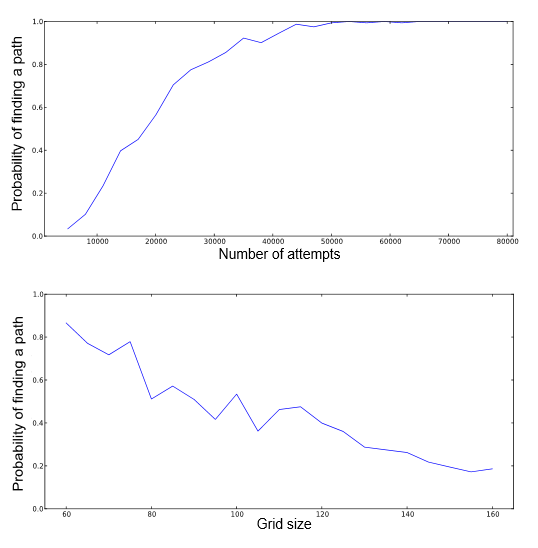
\includegraphics[width=1.0\linewidth]{Tremblay2013.png}
	\caption{ Performance analysis of Tremblay~\textit{et al}'s~\cite{Tremblay2013} RRT when running on a Metal Gear Solid level~\cite{game:MetalGearSolid}.}
	\label{TremblayRRT}
\end{figure} 

\begin{figure}[h]
	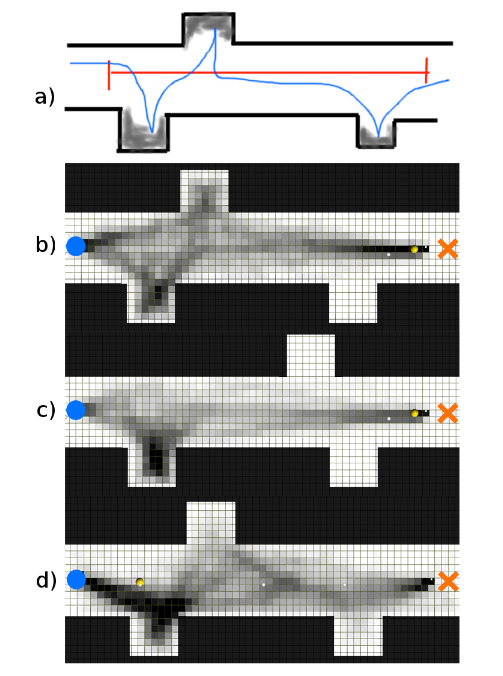
\includegraphics[width=1.0\linewidth]{TremblayHeatMap.png}
	\caption{Heat maps of a single level where the design has been changed each time \cite{Tremblay2013}.}
	\label{TremblayHeatMap}
\end{figure} 

Tremblay~\textit{et al}~\cite{Tremblay2014} again look at the use of search algorithms for use in game development. This work builds on their 2013 paper on RRT in stealth games. As previously mentioned in section \ref{A*PF} they look at the use of A*, MCTS and RRT to visualise player behaviour in platform games similar to Bauer ~\cite{Tremblay2014}~\cite{bauer2012}.  RRT is limited to drawing straight lines between the nodes, as straight lines are not always possible in RRT Tremblay~\textit{et al}~\cite{Tremblay2014} also use either A* or MCTS to find a path to the node and ensure that it is reachable.
While A* is consistently fast with high success rates, RRT has varying results. RRT using MCTS for motion planning varied between 35 and 84 percent success rates and had the longest run times. In comparison, RRT with A* motion planning consistently had a success rate over 60 percent. However, the run times for this combination varied. 
Both of Tremblay~\textit{et al}'s~\cite{Tremblay2014,Tremblay2013} papers showed that a potential issue with the use of RRT is that it may not find a path. Both papers ran RRT combinations over 1000 times. In comparison this paper will run RRT at run time and will only run the algorithm once unless an RRT variant such as RRT* is used. If a path is not found a tree will still be produced and visualised so may still influence players.

Section~\ref{VisualisingAI} will look at Third Eye Crime in more detail for its use of AI visualisation. However, it also uses visualisation of enemy paths as an important mechanic~\cite{Isla2014, game:ThirdEyeCrime}.  Isla~\cite{Isla2014} uses Occupancy Maps to show where the enemy NPC thinks the player could be. Occupancy or Influence Maps do not produce a path instead they show the probability of the player being in different locations across the map~\cite{Isla2014, Miles2006}. Isla used Occupancy Maps to show where the enemy AI thinks the player currently is. The enemy then moves to investigate that area reducing the probability of the player being there.  Similarly, Miles and Louis~\cite{Miles2006} also used influence maps. While their example is specific to \textit{Real Time Strategy} (RTS) games, like Isla they used Occupancy Maps.  They used them as a base for A* path-finding instead of A* using the map itself for path-finding.


\subsection{Foregrounding and Visualising AI} \label{VisualisingAI}
Most modern digital games make use of AI.  However, it is rarely foregrounded or visualised in those games. Treanor~\textit{et al}~\cite{treanor2015} say that often the design of AI in games is to fit the game and complement game play. These AI are supporting the game play rather than being central to it.

Treanor~\textit{et al}~\cite{treanor2015} surveyed many games that foreground or visualise AI in different ways.   From this they propose a series of design patterns for foregrounding AI in digital games. 
The two design patterns relevant to this project are ``AI as a Villain" and ``AI is Visualised".  They describe the first pattern as having the AI try to not outright defeat the player. Instead it is designed to create an experience like in the game Alien Isolation~\cite{treanor2015,game:AlienIsolation}.  In Alien Isolation the enemy AI hunts the player. This is foregrounding as the player must observe the AI and learn how to avoid it. There is also some visualisation as the player has a scanner that will inform them of the enemy's position. 

This paper will use the ``AI as a villain" pattern as each enemy NPC will have their path-finding visualised around them. The players will have to consider this when exploring a level so they do not get attacked by the enemy. The use of this pattern will also aim to have a NPC that creates an experience rather than one that will always find the player, similar to Alien Isolation~\cite{game:AlienIsolation,treanor2015}. While the player will not want to be caught by the enemy NPC they may want it to chase them so they can learn its patterns or lead it away from other enemies to make it easier to attack. 

The second relevant design pattern is ``AI is Visualised".  This is where there is a visual representation of the AI's state or decision making in the game~\cite{treanor2015}. Most games hide this from the player but this design pattern visualises it making it mechanic.  
The example given by Treanor~\textit{et al}~\cite{treanor2015} is the game Third Eye Crime.  Third Eye Crime is a game that follows the ``AI is Visualised" design pattern~\cite{Isla2014,game:ThirdEyeCrime}. The game uses probabilistic object tracking through Occupancy Maps. The game uses Occupancy Maps to display where the enemy thinks the player could be in the map. As the enemy moves around the map it removes areas where the player is not from the Occupancy Map~\cite{Isla2014}.  Generally stealth games involve avoiding enemies.  This design encourages the player to trigger the mechanic, allowing them to use the visualisation to mislead and avoid the enemy~\cite{Isla2014,game:ThirdEyeCrime}. 

\begin{figure}[h]
	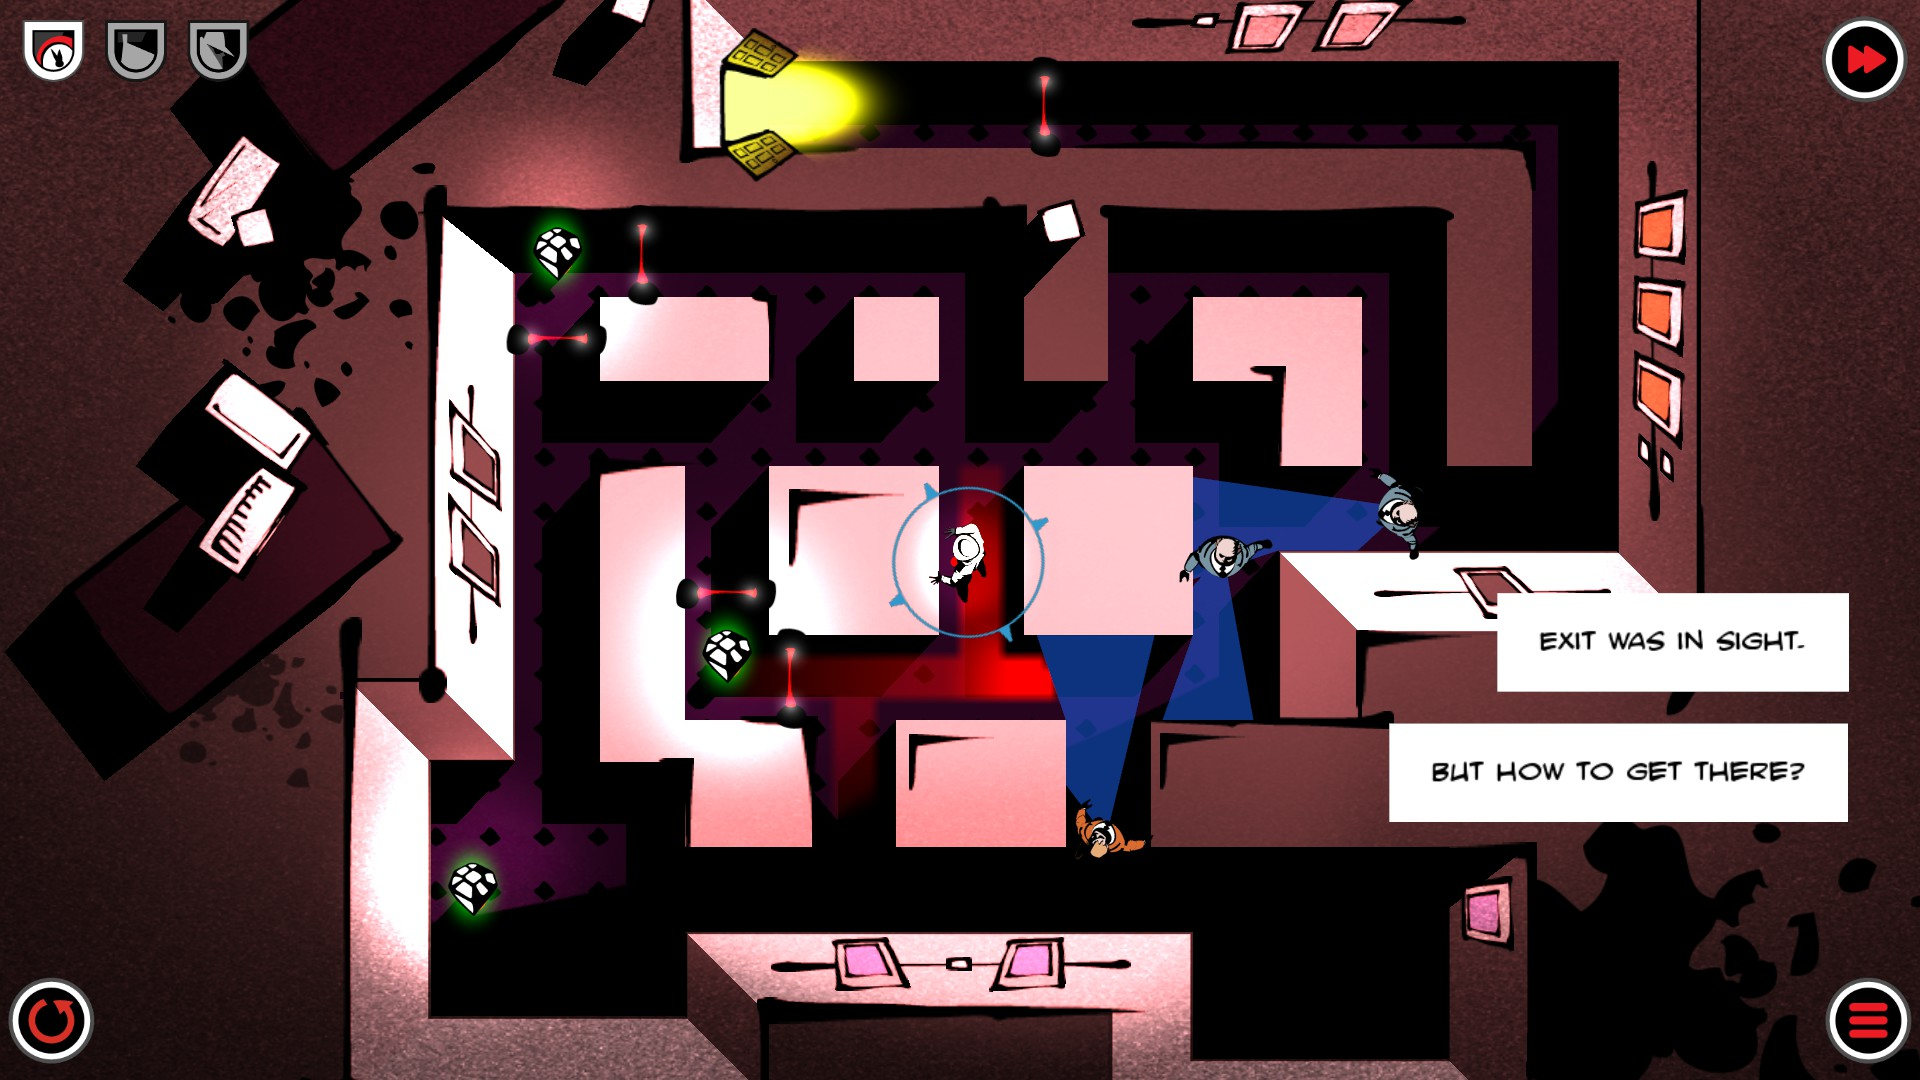
\includegraphics[width=1.0\linewidth]{ThirdEyeCrime.jpg}
	\caption{ A screen-shot from Third Eye Crime~\cite{game:ThirdEyeCrime}.}
	\label{image:ThirdEyeCrime}
\end{figure}  

This pattern is relevant to this project as the enemy NPC will have RRT path-finding visualised around it allowing the player to see where the enemy is searching and decide how to overcome or outsmart it.

% Visualising in general
While Haworth~\textit{et al}~\cite{Haworth2010} do not visualise an AI decision making process they do visualise the possible decisions available to the player in a game on a tree structure.   They research visualising decision trees in a game to see what effect it had on game play and the analytical reasoning of children.  
Their study did not come to any definite conclusions. However, their results suggest that the trees aided players as in the later levels of the game the children without the visualised decision tree struggled to beat the game. However, they noted this could also be due to unbalanced difficulty in the later levels. This makes the usefulness of the visualised tree questionable in this example.  

A potential issue with this study is that Haworth~\textit{et al}~\cite{Haworth2010} only tested the tree on a simple 2-Dimensional maze game for school children. Of these children only a few had experienced playing digital games before.  This could mean that the data is not relevant for 3D games or games available to buy on the market.  In contrast, Isla's~\cite{Isla2014} visualised Occupancy Maps are in the game Third Eye Crime which is available for purchase on Steam, IOS and Android~\cite{Isla2014,game:ThirdEyeCrime}.

Like Haworth~\textit{et al}~\cite{Haworth2010}, Bauer~\textit{et al}~\cite{bauer2012} also research visualising tree structures~\cite{bauer2012}. However, they used RRT which is an AI technique.

Another use of visualisation, mentioned in earlier sections, is in game design. Often to check player behaviour in player testing or to aid the design of levels~\cite{Nelson2011,bauer2012,Tremblay2013,Tremblay2014}. 

\subsection{Exploring Game Environments} \label{Exploring}
% Wayfinding
One method of guiding players through games is to use way-finding. Way-finding in games is often architectural differences or visual cues in the environment that will guide the player to an area of interest~\cite{si2017,Bacim2008}. Way-finding cues are often subtle cues in the environment such as ivy growing up a wall to suggest the player can climb there.

The intention of visualising path-finding in this project is not to guide the players. However, like Si \textit{et al}~\cite{si2017} it will observe how players navigate and explore levels and whether, like the presence of way-finding cues, it affects player behaviour. 
Moura and Bartram~\cite{moura2014} investigate the effects of different way-finding cues on players. They looked at methods used in AAA games and mimicked them in their own game. Their results show that the absence of way-finding cues was obvious to players. In contrast, the version with way-finding cues did not have enough cues to sufficiently guide the player. These results suggest that way-finding cues alone may not be enough to guide the player. They concluded that there is a need for more research as the results were inconclusive. 

While this project focuses on enemy NPC path-finding this could be another interesting application of path-finding and visualisation. The path-finding could remain hidden from the player, as it normally is in digital games, but way-finding cues could be placed based off the path. This could then subtly guide the player through the game.

% Player Exploration
Si \textit{et al}~\cite{si2017} investigated how players explore virtual environments. While their experiments were specific to Real Time Strategy (RTS) games the results may apply to other game types. Si~\textit{et al}~\cite{si2017} say that three common types of spatial exploration are; environment mapping, bonus item collecting and location/landmark discovery. The relevant exploration type for this project is spatial mapping. Firstly, as it is what the enemy NPC will be doing.  Secondly, as it is the player behaviour that is being measured by the logging tool in the software.

A paper looked at in section \ref{VisualisingAI} was Haworth~\textit{et al}'s ~\cite{Haworth2010} study. While they did not look at player exploration the game they used involved a map where participants had to explore a maze. Participants which had the decision tree visualisation found it easier to navigate the maze. While Moura and Bartram~\cite{moura2014} suggested way-finding alone was not enough to guide a player this suggests that visualisation could aid the exploration process~\cite{Haworth2010}.

\section{Methodology} \label{methodology}
The proposed research question is: how does visualising path-finding in a NPC affect how players explore a game level? The hypothesis drawn from this question are listed in subsection \ref{hypothesis}.  For an effect size of 0.4 in this study at least 52 to partcipants were needed. 

\textbf{POWERANALYSIS SCREENSHOT}

All?? players were university students, most from game developement related courses. $\to$ This may have influenced the results as students studying game developement using the Unity engine are likely to be to guess what the visualisations are showing??
Another potential issue is that some partcipants may have user tested a variation of the game before and therefore known parts of the level layouts which could influence how much they explored. 


\subsection{Hypothesis:} \label{hypothesis}
\begin{table*}[h]
	\centering
	\caption{Hypothesis}
	\label{table:Hypothesis}
	\def\arraystretch{1.5}
	\begin{tabular}{|c|p{7.5cm}|p{7.5cm}|}
		\hline
		 & \textbf{Hypothesis}& \textbf{Null Hypothesis} \\
		\hline
		1 & Visualising path-finding has an effect on the percent of the level the participant explores.
			& Visualising path-finding has no effect on the percent of the level the participant explores.
		\\ \hline
		
		2 & Visualising RRT path-finding has an effect on the percent of the level the participant explores.
		& Visualising RRT path-finding has no effect on the percent of the level the participant explores.
		\\ \hline
		
		3 & Visualising Unity navmeshes has an effect on the percent of the level the participant explores.
		& Visualising Unity navmeshes has no effect on the percent of the level the participant explores
		\\ \hline
		
		4 & Visualising RRT has an effect on the length of time the participant spends in the level. 
		& Visualising RRT has no effect on the length of time the participant spends in the level. 
		\\ \hline
		
		5 & Visualising Unity navmeshes has an effect on the length of time the participant spends in the level. 
		& Visualising Unity navmeshes has no effect on the length of time the participant spends in the level.
		\\ \hline
		
		6 & In comparison to RRT visualisation visualising Unity navmeshes has an effect on the percent of the level the participant explores.
		& In comparison to RRT visualisation visualising Unity navmeshes has no effect on the percent of the level the participant explores.
		\\ \hline
		
		7 &  In comparison to RRT visualisation visualising Unity navmeshes has an effect on length of time the participant spends in the level. 		
		&   In comparison to RRT visualisation visualising Unity navmeshes has an effect on length of time the participant spends in the level. 	
		\\ \hline
		
		8 &   The visualisation of  Unity navmeshes is comprehensible to players.
		&  The visualisation of  Unity navmeshes is not comprehensible to players.
		\\ \hline
		
		9 &  The visualisation of  RRT pathfinding is comprehensible to players.
		&  The visualisation of  RRT pathfinding is not comprehensible to players.
		\\ \hline
			
		10 &  The comprehensibility of  the visualisation of RRT pathfinding is no different to Unity navmesh visualisation to players.
		&  The comprehensibility of  the visualisation of RRT pathfinding is different to Unity navmesh visualisation to players.
		\\ \hline
	\end{tabular}
\end{table*}
Table \ref{table:Hypothesis} shows the hypothesis being tested in this experiment. The methodology that will be used to test these hypotheses will be play testing and a questionnaire. This will require human participants for both parts. Ethics approval for this methodology was gained from Falmouth University’s Research Ethics board.

The game the enemy NPC will be tested in is a 3D metroidvania game which has a focus on exploration. A metroidvania game is an action-adventure game with a focus on exploration to discover new areas and power ups. Players will be given one of the game variations to play and then asked to complete a questionnaire on their experience. The game will also log the player's position at regular intervals to calculate what percent of the level they explore. How long a participant spends exploring the level will also be logged.

\subsection{Playtest Variations}
Players were all randomly assigned one of the four games variations shown in table \ref{table:PlaytestVariations}. 

\begin{table}[H]
	\centering
	\caption{Playtest Variations}
	\label{table:PlaytestVariations}
	\def\arraystretch{1.5}
	\begin{tabular}{ |l|l|l|}
		\hline
			  							& \textbf{Unity Navmesh}& \textbf{RRT} \\
		\hline
		\textbf{Hidden Path-finding}	& Variation 1			& Variation 3 \\
		\hline
		\textbf{Visualised Path-finding}& Variation 2		  	& Variation 4 \\
		\hline
	\end{tabular}
\end{table}

During the play tests players will be randomly assigned either RRT or navmesh pathfidning variations of the game. The players will be asked to play two versions of the game: one with visualisation and one without. Both versions they play will be using the same pathfinding method.

A-B testing will be used on participants. A-B testing is where each participant will be assigned a version of the game to play~\cite{Hynninen2014}. In this case to prevent them from guessing what the goal of the play test is. 

For the first round of play testing each participant will be asked to play two versions of the game 

The software will log the player's position in the level throughout their play test. This data will be exported in a .CSV every second. Varying the export rate is unlikely to provide data of interest as the focus is on time spent in a level and how much was explored. 

The exported data will then be analysed using R\footnote[2]{R Available: https://www.r-project.org/}. Wallner says heat maps are useful as they are easy to generate and easy to discern patterns from~\cite{Wallner2015}.  Tremblay~\textit{et al}~\cite{Tremblay2014} also used heat maps on their RRT visualisations. They used them as part of their tool for level designers to use to see where players could go and the effects of them altering the level design which can be seen in Figure \ref{TremblayHeatMap}. Here they will only be used for analysis and to assist in finding noticeable patterns.

Other statistical analysis in R will be generated to support the heat maps. T-Tests will be performed to compare the data on the null hypothesis and the sets of data on hypotheses 1 to 3.
 
After completing a play test of the game participants will be asked to complete a questionnaire on their experience.

\subsection{Questionnaire} \label{Questionnaire}

Alongside play testing participants will also be asked to fill out a questionnaire on the game online using Google Forms. Nordin \textit{et al}~\cite{nordin2014} say that questionnaires are vital for understanding how players feel when playing digital games~\cite{nordin2014,Denisova2016}. They can also help give uniformity and consistency to the data gathered from participants~\cite{Denisova2016}.

Questionnaires are also beneficial as they can prompt players to give answers they may not have given spontaneously. The two options here are to either create a questionnaire specifically for the experiment or to use an existing one. There are a wide variety of questionnaires that already exist to measure players experiences in play testing~\cite{nordin2014,Jennett2008}. These come with the benefit of being more likely to be thoroughly tested such as the \textit{Immersive Experience
Questionnaire} (IEQ) which uses Likert scale responses or Yee's taxonomy~\cite{nordin2014,Jennett2008, Yee2006, Yee2012}.
 
However, Nordin \textit{et al}~\cite{nordin2014} say there are many issues with using preexisting questionnaires. Firstly, many of these questionnaires are not readily available. Another issue is that not all questionnaires have been thoroughly checked for validity. There is also the potential issue of a researcher not fully understanding the questions put forward by another researcher or they may not understand what data that question is intended to get.

Another potential issue with a questionnaire is self report bias. Some of the hypothesis being tested relate to the player being confused or not understanding the visualisations. Players are unlikely to admit to not understanding the game making the data gained invalid. \textbf{FIND REF}

Most of the hypotheses here can be tested using the quantitative data from the play tests. However, some require qualitative data so a questionnaire will be necessary. 
Yee's questionnaire for player taxonomy's will be used in combination with questions based of the hypotheises that require qualitative data.

\textbf{NEW STUFF} \\
Looked at Bartle not validated \cite{Bartle1996} but used: 

\section{Software Development} \label{softdev}
The software used to develop the play testing software was Unity 5.6.3f1\footnote[3]{Unity 5.6 Available: https://unity3d.com/get-unity/download/archive} and Visual Studio Community 2017  15.5.4\footnote[4]{Visual Studio Community 2017 Available: https://www.visualstudio.com/downloads/}.

The analysis was carreid out in R version 3.4.?? in R Studio.

The development cycle of this software was a combination of the Incremental and Agile software developement cycles. Basic features were developed and then iterated on until the software was useable for play testing. Trello\footnote[5]{Trello Available: https://trello.com/} was used to manage tasks.

\section{Software Testing} \label{softtest}
To test the play-testing a series of simple bots were developed to move though the level to test various functionality.

\todo[inline]{Bot runs forward/back/jumps checks metrics are recorded.}

\subsection{Doors}
The first bot was to test whether the doors recorded whether the player had moved through them. Whether a door has been walked through it used to determine what percent of the level the player explored.
The test was a bot moving through the door and checking that the GameState class recorded it.

\todo[inline]{SCREENSHOTS OF BOT AND DOOR AND GAMESTATE.}

\subsection{Timer and Data Export}
The second bot was to check whether the software could successfaully export the necessary data to a .csv file. This bot is based of the door bot, the only difference is that it closes the game at the end to trigger the data export.  

\todo[inline]{SHOW TIMER ON SCREEN AND EXPORTED DATA.}

\subsection{Visualisations}
The final test was whether the path-finding visualisation worked as intended. This did not require a bot it can be seen tested by observing the scene in Unity. Figure \ref{image:navmeshVisuals} shows the visualisation of the Unity navmesh working in engine.  Figure \ref{image:RRTVisuals} shows the visualisation of the RRT path-finding working in engine.

\begin{figure}[h]
	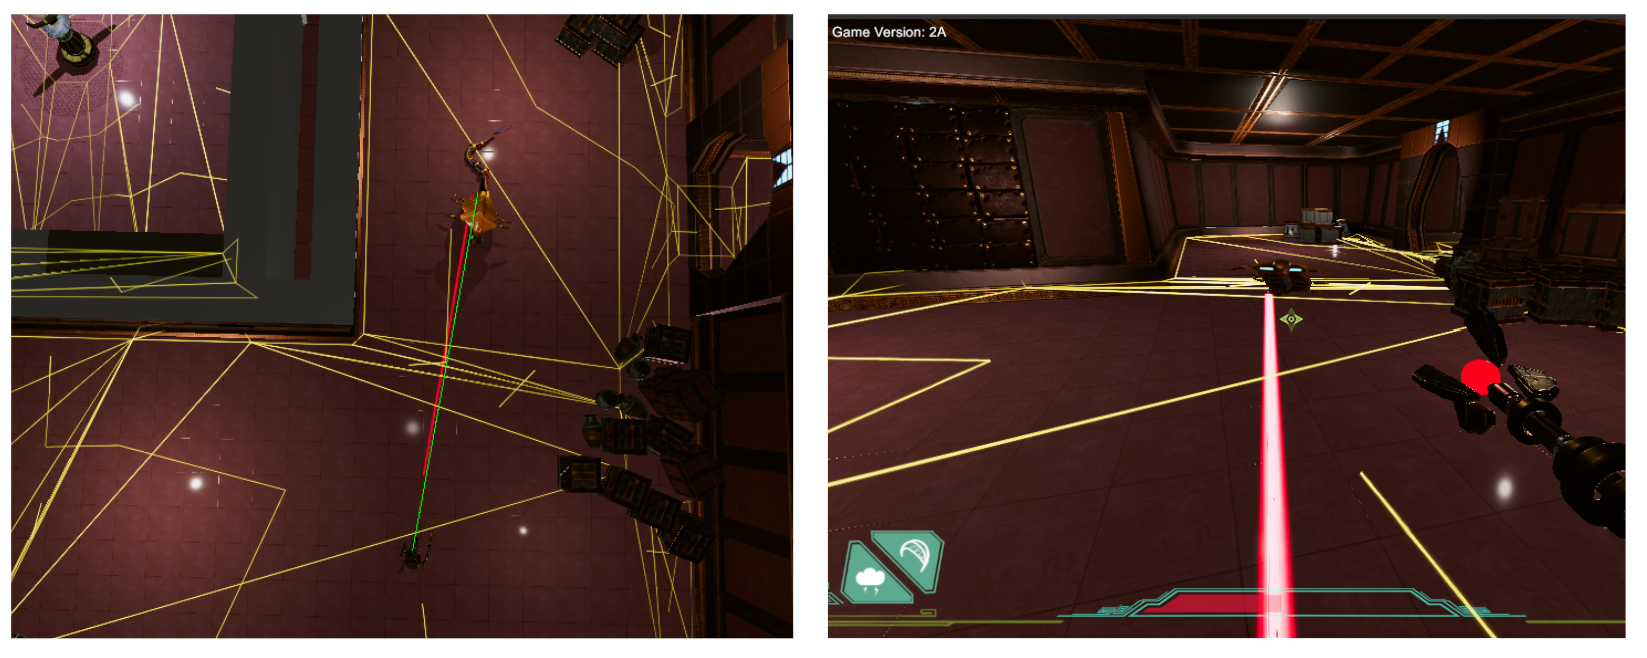
\includegraphics[width=1.0\linewidth]{NavmeshVis.png}
	\caption{The navmesh visualisations shown both in editor and in scene.}
	\label{image:navmeshVisuals}
\end{figure}  


\begin{figure}[h]
	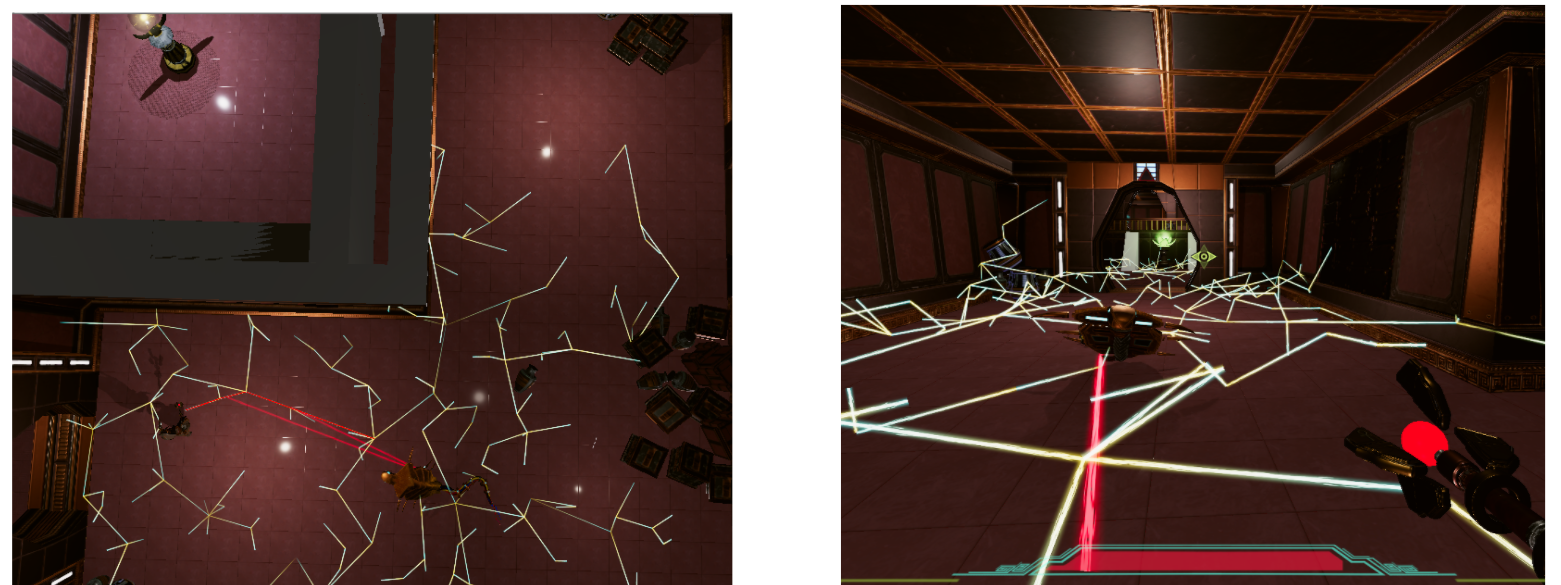
\includegraphics[width=1.0\linewidth]{RRTVis.png}
	\caption{The RRT visualisations shown both in editor and in scene.}
	\label{image:RRTVisuals}
\end{figure}  

\section{Analysis and Interpretation}

\todo[inline]{Data collected, detail on that.}
\todo[inline]{Analysis of data.}
\todo[inline]{Interpretation.}

\section{Conclusion} 
\todo[inline]{NEEDS UPDATING BASED OFF DATA}
In conclusion, while the use of RRTs is more frequent in robotics than digital games its use appears feasible in this project. Its past use in game design tools shows that clustering can make the output understandable to the user. However, the need of optimisations such as RRT* or the use of A* may arise to produce a shorter path or to find any path. 

Visualisation and foregrounding of AI have been successfully used before suggesting that it can used here. Finally, previous studies have looked at way-finding and player exploration. These suggest that environmental factors in digital environments do have some effect on player exploration.


% references section
\bibliographystyle{IEEEtran}
\bibliography{references}

% Appendices

 \appendices
 \section{First appendix}
 Appendices are optional. Delete or comment out this part if you do not need them.

% that's all folks
\end{document}
